% This is the University of Chicago Graham School Master of Science in Analytics
% template. Much of it is based on the Reed College LaTeX thesis template.
% Most of the work for the Reec College template was done by Sam Noble (SN),
% Later comments etc. by Ben Salzberg (BTS).
% Additional restructuring and APA support by Jess Youngberg (JY).
% Justin M. Shea (JMS) built on their good open source work.
% Your comments and suggestions are more than welcome:
% please email, them to justinshea@uchicago.edu.
%
% Any line that starts with a percent symbol is a comment.
% They won't show up in the document, and are useful for notes
% to yourself and explaining commands.
% Commenting also removes a line from the document;
% very handy for troubleshooting problems. -BTS
%%
%% Preamble
%%
% \documentclass{<something>} must begin each LaTeX document
% Added by JMS
\documentclass[12pt,oneside]{chicagocapstone}
% END of JMS add
% Packages are extensions to the basic LaTeX functions. Whatever you
% want to typeset, there is probably a package out there for it.
% Check out CTAN to see: http://www.ctan.org/
%%
\usepackage{graphicx,latexsym}
\usepackage{amsmath}
\usepackage{amssymb,amsthm}
\usepackage{longtable,booktabs,setspace}
\usepackage[hyphens]{url}
% Added by CII
\usepackage{hyperref}
\usepackage{lmodern}
\usepackage{float}
\floatplacement{figure}{H}
% End of CII addition
\usepackage{rotating}


% Added by CII (Thanks, Hadley!)
% Use ref for internal links
\renewcommand{\hyperref}[2][???]{\autoref{#1}}
\def\chapterautorefname{Chapter}
\def\sectionautorefname{Section}
\def\subsectionautorefname{Subsection}
% End of CII addition

% Added by CII
\usepackage{caption}
\captionsetup{width=5in}
% End of CII addition

% Added by JMS
\usepackage{mathptmx} % Times New Roman fonts
% End of add by JMS

% Syntax highlighting #22

% To pass between YAML and LaTeX the dollar signs are added by CII
\title{Data Analytics as a Service (DAaaS): Automated \& Intelligent Imputation
Methods for Supervised Machine Learning}
\author{Shahid Barkat, Joseph Kearney}
\date{June, 2019} % The month and year that you submit your FINAL draft)
\division{Graham School}
\advisor{Dr.~Arnab Bose}
\institution{University of Chicago}
\degree{Master of Science in Analytics}
\altadvisor{Dr.~Sema Barlas}
% End of CII addition

\department{Continuing Liberal and Professional Studies}

% Added by CII
%%% Copied from knitr
%% maxwidth is the original width if it's less than linewidth
%% otherwise use linewidth (to make sure the graphics do not exceed the margin)
\makeatletter
\def\maxwidth{ %
  \ifdim\Gin@nat@width>\linewidth
    \linewidth
  \else
    \Gin@nat@width
  \fi
}
\makeatother

\renewcommand{\contentsname}{Table of Contents}
% End of CII addition

\setlength{\parskip}{0pt}

% Added by CII
  %\setlength{\parskip}{\baselineskip}
  \usepackage[parfill]{parskip}

\providecommand{\tightlist}{%
  \setlength{\itemsep}{0pt}\setlength{\parskip}{0pt}}


\Abstract{
The researchers develop and maintain an open-source, Python-based
package named Autoimpute to address one of the most common nuisances in
machine learning -- datasets with missing values. The package implements
numerous imputation algorithms and extends common supervised machine
learning methods to handle multiply imputed datasets. Autoimpute treats
missing data as a first-class citizen in the Python world, making
imputation familiar to Python developers and easy to use for those new
to the language. Ultimately, the package provides users an end-to-end
framework that covers missing data exploration to imputation analysis.

\bigskip  \bigskip
\bigskip

\textbf{Keywords}: Missing Data; Imputation; Python; Autoimpute Package;
Machine Learning; Bias/Variance Analysis; Fractional Factorial Design,
SciKit Learn; Pandas
}

% Added by JMS
\Executive{
This research develops an end-to-end methodology to address one of the
most common nuisances in machine learning -- datasets with missing
values. It approaches incomplete datasets with four objectives: describe
and visualize the extent of the missing value problem; examine factors
related to missingness; develop methods to impute missing data; and
measure the impact of imputation on inference derived from supervised
learning, specifically linear and logistic regression.

To meet these objectives, the researchers develop and maintain an
open-source, Python-based package named Autoimpute. The package works
with pandas DataFrames and implements numerous imputation algorithms,
which the authors cover later in this report. Autoimpute also extends
common supervised machine learning methods to handle imputed datasets.
The package includes linear and logistic regression specifically
designed for multiply imputed data as well as methods to assess the
impact of imputation on parameter inference from these analysis models.
Further, Autoimpute follows the API design of popular Python machine
learning package, scikit-learn. Its ``Imputers'' integrate nicely with
scikit-learn machine learning pipelines.

Autoimpute treats missing data as a first-class citizen in the Python
world, making imputation familiar to Python developers and easy to use
for those new to the language. The package incorporates the four
objectives outlined above and provides users an end-to-end framework
that covers missing data exploration to imputation analysis. In doing
so, Autoimpute remains flexible, yielding users as much control and
complexity as they would like while they grapple with missing data.
}
% End of JMS add

\Acknowledgements{

}

\Dedication{

}

\Preface{

}


% End of CII addition
%%
%% End Preamble
%%
%
\begin{document}

% Everything below added by CII
  \maketitle

\frontmatter % this stuff will be roman-numbered
\pagestyle{empty} % this removes page numbers from the frontmatter


%% Reorganized by JMS
  \begin{abstract}
    The researchers develop and maintain an open-source, Python-based
    package named Autoimpute to address one of the most common nuisances in
    machine learning -- datasets with missing values. The package implements
    numerous imputation algorithms and extends common supervised machine
    learning methods to handle multiply imputed datasets. Autoimpute treats
    missing data as a first-class citizen in the Python world, making
    imputation familiar to Python developers and easy to use for those new
    to the language. Ultimately, the package provides users an end-to-end
    framework that covers missing data exploration to imputation analysis.
    
    \bigskip  \bigskip
    \bigskip
    
    \textbf{Keywords}: Missing Data; Imputation; Python; Autoimpute Package;
    Machine Learning; Bias/Variance Analysis; Fractional Factorial Design,
    SciKit Learn; Pandas
  \end{abstract}
 % Added by JMS
  \begin{executive}
    This research develops an end-to-end methodology to address one of the
    most common nuisances in machine learning -- datasets with missing
    values. It approaches incomplete datasets with four objectives: describe
    and visualize the extent of the missing value problem; examine factors
    related to missingness; develop methods to impute missing data; and
    measure the impact of imputation on inference derived from supervised
    learning, specifically linear and logistic regression.
    
    To meet these objectives, the researchers develop and maintain an
    open-source, Python-based package named Autoimpute. The package works
    with pandas DataFrames and implements numerous imputation algorithms,
    which the authors cover later in this report. Autoimpute also extends
    common supervised machine learning methods to handle imputed datasets.
    The package includes linear and logistic regression specifically
    designed for multiply imputed data as well as methods to assess the
    impact of imputation on parameter inference from these analysis models.
    Further, Autoimpute follows the API design of popular Python machine
    learning package, scikit-learn. Its ``Imputers'' integrate nicely with
    scikit-learn machine learning pipelines.
    
    Autoimpute treats missing data as a first-class citizen in the Python
    world, making imputation familiar to Python developers and easy to use
    for those new to the language. The package incorporates the four
    objectives outlined above and provides users an end-to-end framework
    that covers missing data exploration to imputation analysis. In doing
    so, Autoimpute remains flexible, yielding users as much control and
    complexity as they would like while they grapple with missing data.
  \end{executive}
 % End of JMS




  \hypersetup{linkcolor=black}
  \setcounter{tocdepth}{2}
  \tableofcontents

  \listoffigures

  \listoftables

%% END of Reorganization by JMS

\mainmatter % here the regular arabic numbering starts
\pagestyle{fancyplain} % turns page numbering back on

\chapter*{Introduction}\label{introduction}
\addcontentsline{toc}{chapter}{Introduction}

The researchers develop and maintain an open-source, Python-based
package named \texttt{Autoimpute} to address one of the most common
nuisances in machine learning -- datasets with missing values. The
package implements numerous imputation algorithms and extends common
supervised machine learning methods to handle multiply imputed datasets.
\texttt{Autoimpute} treats missing data as a first-class citizen in the
Python world, making imputation familiar to Python developers and easy
to use for those new to the language. Ultimately, the package provides
users an end-to-end framework that covers missing data exploration to
imputation analysis.

\section*{Problem Statement}\label{problem-statement}
\addcontentsline{toc}{section}{Problem Statement}

Machine learning models rely entirely on the data they are provided, and
most require that the underlying dataset be complete. In reality,
however, many real-world datasets are incomplete, containing missing
values for the response variable and one or more of the features
collected. As a result, the machine learning practitioner must decide
what to do about missing data. The way in which the practitioner handles
missing data greatly affects the interpretability of and results from
the machine learning models the practitioner builds and deploys.

The challenge of handling missing data has inspired numerous imputation
methods, each of which has its advantages and disadvantages depending on
the nature of the missing data and the machine learning task at hand.
Unfortunately, the existence of multiple imputation methods does not get
the machine learning practitioner any closer to handling missing data.
First, imputation methods can be challenging to understand and
computationally expensive to implement. Next, no global criteria or
metric exists to select the optimal imputation method given a dataset
with missing values. Even if a practitioner successfully implements
imputation methods, he or she has no structured way to evaluate how well
imputation performs or how imputation affects supervised models
downstream built upon imputed data.

Because handling missing data is quite complex, most statistical
packages simply remove records with missing data so that machine
learning models can execute. While this option is simple to implement
and enables models to run, it generally comes with numerous undesirable
side effects if data is not missing completely at random (MCAR). This
subject is explored further in the background section of this paper.
However, in practice, real-world data is rarely MCAR, so models should
generally avoid discarding missing records. Extensions in software
packages do exist to implement imputation methods automatically. That
being said, the practitioner still must decide which method to
implement, explain why an imputation method is optimal, and evaluate how
the optimal imputation method affects models trained on imputed data.

\section*{Research Purpose}\label{research-purpose}
\addcontentsline{toc}{section}{Research Purpose}

This research aids the machine learning practitioner by bringing more
clarity to the imputation process, making imputation methods more
accessible and comparable, and measuring the impact imputation methods
have in supervised regression and classification models. This research
strives to not just automate imputation but also develop an open-source
framework to structure and evaluate imputation methods within a
supervised machine learning process.

To address this purpose, this research specifies four objectives:
\begin{enumerate}
\def\labelenumi{\arabic{enumi}.}
\tightlist
\item
  Assess the extent of the missing data problem with descriptive and
  visual measures\\
\item
  Examine the factors related to the missingness of data\\
\item
  Deploy imputation methods and select the most appropriate
  methodology\\
\item
  Measure the impact of imputation to the fit, stability, bias, and
  variance of parameters derived from supervised models built on imputed
  data
\end{enumerate}
The researchers meet these objectives by developing an open-source
Python package that can generalize across cross-sectional and
time-series datasets. Any data science professional can deploy or reuse
components of the package itself. Eventually, the researchers will
accept contributions from the open source community as well.

\hypertarget{background}{\chapter*{Background}\label{background}}
\addcontentsline{toc}{chapter}{Background}

One must understand what missingness means and why it exists before one
decides how to handle it. The authors explore concepts related to
missingness using a motivating example. For an experiment, assume that a
random sample of measurements is collected from thousands of weigh
scales. Also assume each weigh scale in the experiment may fail to
produce measurements for three separate reasons. First, a scale might
run out of batteries, in which case all measurements from that scale
cease for a given period of time. Next, a scale may fail more frequently
for heavier objects or items over a certain weight threshhold. And
finally, a scale may stop reporting measurements when placed on a soft
surface instead of a hard one (Van Buuren, 2018, ch.~1.2).

As a result of these scenarios, the random sample collected likely has
many instances in which weight measurements are unobserved. How
missingness in this sample is handled moving forward will depend on
characteristics of the missing data itself and the process that
generated missingess. The authors devote the rest of this section to
concepts related to the nature of missingness and how it is handled. The
authors refer back to this example to make concepts more concrete.

\section*{Basic Terminology and Notation}\label{background-basic-terms}
\addcontentsline{toc}{section}{Basic Terminology and Notation}

Before diving into concepts related to missingness, the authors
establish notation used throughout this text. In doing so, the authors
also introduce some basic terminology. This research follows the
notation Van Buuren uses in the second edition of his book, Flexible
Imputation of Missing Data. For more information, refer to Appendix B,
which collects and summarizes the notation seen throughout this
research.

In the introductory example, weigh scales produce a set of \(n\)
measurements, some of which may be missing weight. \(Y\) denotes the
\(n\) x \(p\) matrix that contains the \(n\) measurements and the \(p\)
variables recorded along with the measurements. The surface of the scale
(hard or soft) is an example of a discrete variable in \(p\), while the
weight measurement itself is a continuous variable in \(p\). We can
retrieve an observation within \(Y\) by specifying the row and column
index corresponding to the observation's cell. To do so, we use the
notation \(y_{ij}\), where \(i\) represents the row and \(j\) represents
the column associated with a scalar \(y\) in matrix \(Y\).

\(Y\) itself represents the hypothetically complete data (Van Buuren,
2018, ch.~2.2.3), which is comprised of \(Y_{obs}\) and \(Y_{mis}\).
\(Y_{obs}\) represents each row \(Y_i\) out of \(n\) records that have
known values for each column \(Y_j\) in \(p\). \(Y_{mis}\), on the other
hand, contains records with missing observations across any of the
columns in \(p\). Note that \(Y = (Y_{obs}, Y_{mis})\). The
hypothetically complete data equals the conjoined observed and missing
data matrices.

It is convenient to store whether or not a cell in \(Y\) is missing in a
separate matrix \(R\). Therefore, \(R\) is an \(n\) by \(p\) matrix
where all entries \(r_{ij} \in {0, 1}\). Any observation \(r_{ij}=1\)
corresponds to a known value for \(y_{ij}\). On the contrary, any
observation \(r_{ij}=0\) corresponds to a missing value for \(y_{ij}\).
\(R\) is commonly referred to as the \textbf{missing indicator matrix},
while \(Y\) is the \textbf{complete data matrix} (Van Buuren, 2018,
ch.~2.2.3).

\section*{Missing Data Mechanism}\label{background-missing-data-mech}
\addcontentsline{toc}{section}{Missing Data Mechanism}

Each of the three scenarios discussed above causes a given weigh scale
to produce missing data, but the underlying reason for missingness is
quite different in each case. Donald Rubin describes the ways in which
data can be missing (Rubin, 1976). According to Rubin (as cited in Van
Buuren, 2018, ch.~1.2), every observation in a dataset has some
probability of being missing. The process that governs these
probabilities is called the \textbf{missing data mechanism} (Rubin, as
cited in Van Buuren, 2018, ch.~1.2). The missing data mechanism
generates a statistical relationship between observations and the
probability of missing data (Nakagawa, 2015, pg. 83). The
\textbf{missing data model} is the function that formalizes that
statistical relationship (Van Buuren, 2018, ch.~2.2.4). These
statistical relationships fall into one of three categories, each of
which represents a different missing data mechanism (Rubin, as cited in
Van Buuren, 2018, ch.~1.2).

The general expression for the missing data model is defined as:

\[P(R|Y_{obs}, Y_{mis},\psi)\]

\(\psi\) cointains the parameters of the missing data model. This
expression notes that the probability of missingness \(P(R=0)\) within a
dataset depends on the observed data, the missing data, and the missing
data model's parameters. (Van Buuren, 2018, ch.~2.2.4). From another
lense, this expession states that the missing data model is the
distribution of the missingness indicator conditional on the observed
data, the missing data, and the parameters of the missing data model.

The missing data model is the function that formalizes the statistical
relationship governed by a missing data mechanism. The next section
examines the manifestation of the missing data model under each
mechanism.

\subsection*{MCAR, MAR, and MNAR}\label{background-mcar-mar-mnar}
\addcontentsline{toc}{subsection}{MCAR, MAR, and MNAR}

Rubin popularized names for the three categories that represent the main
missing data mechanisms:
\begin{itemize}
\tightlist
\item
  \textbf{Missing Completely at Random (MCAR)}
\item
  \textbf{Missing at Random (MAR)}
\item
  \textbf{Missing Not at Random (MNAR)}
\end{itemize}
In this research, the authors refer to each category by its abbreviated
label. The subsections below examine each category in more detail.

\subsubsection{Missing Completely at Random
(MCAR)}\label{missing-completely-at-random-mcar}

MCAR is the first of the three missing data mechanisms. MCAR assumes
missing values in the underlying dataset have the same probability of
missingness for all cases (Gelman \& Hill, 2017, pg. 530). Thus, MCAR
implies that the probability of missingness within a dataset is
completely unrelated to the data in question or any other observed or
unobserved data. The missing data model associated with MCAR is defined
as:

\[P(R=0|Y_{obs},Y_{mis},\psi) = P(R=0|\psi)\]

Note that the general expression of the missing data model reduces to a
much simpler form. Under MCAR, the probability of data being missing
depends on the parameters of the missing data only and not on the values
of missing data itself or the value of any of the observed data (Van
Buuren, 2018, ch.~2.2.4).

From the weigh scale example, MCAR governs the probability of values
being missing from a scale that runs out of batteries at some point in
time (Van Buuren, 2018, ch.~1.2). For simplicity, assume time is not a
latent variable nor of interest in the data collection process. In this
case then, the missing values produced from the scale do not depend on
the weight of the object in question nor the surface used for the scale,
so the probability a value is missing does not depend on any of the
missing or observed data. Although MCAR is convenient, it is very
restrictive and generally unrealistic, so datasets with missing values
are often not MCAR in the real world (Van Buuren, 2018, ch.~2.2.4).

\subsubsection{Missing at Random (MAR)}\label{missing-at-random-mar}

MAR is the second missing data mechanism. MAR occurs when the
probability a given variable is missing depends on available and
observed information only (Gelman \& Hill, 2017, pg. 530). MAR is a
weaker and more general classification of missingness than MCAR
(Allison, 2012). The missing data model associated with MAR is defined
as:

\[P(R=0|Y_{obs},Y_{mis},\psi) = P(R=0|Y_{obs},\psi)\]

For MAR, the missing data model reduces because the probability of data
being missing depends on the missing data model and the observed data
only. Therefore, \(Y_{mis}\) does not affect the probability of
missingness under MAR.

In the case of the weigh scale, MAR describes missing data that arises
from the scale's placement on hard or soft surfaces. If information
about the surface (hard or soft) is fully observed for each attempted
weight measurement, the probability of missing measurements then depends
on available data - surface type - and thus falls under MAR (Van Buuren,
2018, ch.~1.2). Since MAR is a more general assumption than MCAR, it is
more realistic to encounter in real-world datasets.

\subsubsection{Missing Not at Random
(MNAR)}\label{missing-not-at-random-mnar}

Missing not at random (MNAR) is the final missing data mechanism. MNAR
suggests data's ``probability of being missing varies for reasons that
are unknown to us'' (Van Buuren, 2018, ch.~1.2). As a result, the
missing data model for MNAR does not reduce:

\[P(R=0|Y_{obs},Y_{mis},\psi)\]

Missing data under MNAR may depend on observed and unobserved data, so
the missing data model does not simplify at all. There are two major
sub-categories that capture ``unobserved'' within MNAR. First,
missingness may depend on the actual missing values themselves (Gelman
\& Hill, 2017, pg. 530). When the weight of an object itself is to blame
for a scale's failure to report measurements, the underlying process
falls under this sub-category of MNAR because the probability of weight
being missing is related to weight itself (Van Buuren, 2018, ch.~1.2).
The second type of MNAR covers missingness that depends on unobserved
measurements or latent variables (Gelman \& Hill, 2017, pg. 530). The
weigh scale example proposes three reasons a scale may generate missing
measurements. These reasons do not cover countless other possibilities
for why missing data may occur, such as the brand or age of a given
scale. If the brand or age of a scale contributes to the probability of
missing measurements but data is not available regarding a scale's brand
or age, then the missing data mechanism falls under the second
sub-category of MNAR.

\subsection*{Ignorability}\label{background-ignorability}
\addcontentsline{toc}{subsection}{Ignorability}

The missing data mechanism underpins the assumptions one can make when
handling missing data. The most important assumption is that of
\textbf{ignorability}. Missingness is ignorable ``if it is missing at
random and the probability of a missingness does not depend on the
missing information itself'' (Introduction to SAS, 2017). Therefore, the
missingness within a dataset is said to be ignorable if the underlying
missing data mechanism is MCAR or MAR. MNAR, on the other hand,
constitutes missingness that is non-ignorable.

As Van Buuren Notes, ``the concept of ignorability plays an important
role in the construction of imputation models'' (2018, ch.~2.2.6).
Specifically, ignorability determines whether one can ignore the way in
which data are missing prior to imputing missing data through an
imputation model (Nakagawa, 2015, Pg. 85). As stated in Introduction to
SAS, ``the assumption of ignorability is needed for optimal estimation
of missing information and is a required assumption'' (2017).

To formalize the statements above, consider the general expression for
an imputation model:

\[P(Y_{mis}|Y_{obs}, R)\]

This expression means that the distribution of the missing data depends
on the distribution of the observed data \(Y_{obs}\) and the process
that generated the missing data, \(R\) (Van Buuren, 2018, ch 2.2.6). In
the context of imputation, this expression suggests that the imputed
values are generated conditional on the observed data and missing data
mechanism.

If the missingness is ingorable, then:

\[P(Y|Y_{obs}, R=1) = P(Y|Y_{obs}, R=0)\]

This equality states that the distribution of the data \(Y\) is the same
for both the response (observed) and non-response (missing) groups (Van
Buuren, 2018, ch 2.2.6). Essentially, this equation suggests that
imputation models need not consider the missing data model when creating
imputations for \(Y_{mis}\). As a result, the parameters of the missing
data model, \(\psi\), are not important if the underlying missing data
mechanism is ignorable.

The importance of this equality becomes clear through an example. Take
the weigh scale experiment introduced in the beginning of the
\protect\hyperlink{background}{Background section}. Assume
\(Y_{weight}\) contains weight measurements in \(Y\), and
\(Y_{surface}\) specifies the surface (hard or soft) of the scale
generating weight measurements. The researcher can model weight using
the observed data only within each surface:
\(P(Y_{weight}|Y_{surface}=hard, R=1)\) and
\(P(Y_{weight}|Y_{surface}=soft, R=1)\). If the missing data mechanism
is ignorable, then \(P(Y_{weight}|Y_{surface}=hard, R=1)\) =
\(P(Y_{weight}|Y_{surface}=hard, R=0)\) for hard surfaces and
\(P(Y_{weight}|Y_{surface}=soft, R=1)\) =
\(P(Y_{weight}|Y_{surface}=soft, R=0)\) for soft surfaces. Therefore,
the researcher can draw imputations for weight conditional on observed
data only; he or she does not need to consider the missing data model
within each subgroup, because the distribution for the observed and the
missing data is the same (Van Buuren, 2018, ch.~2.2.6).

If within each surface group the distribution for missing weights
depends further on the actual mass of the object weighed, then the
researcher cannot ignore the missing data model, because imputed values
drawn from the observed data would be systematically different than the
distribution of imputed values drawn when taking the missing data model
into consideration. In this example, if weight were missing for objects
that had a higher weight, imputations drawn from the observed data would
systematically understate the weight of the missing objects regardless
of the surface of the scale if the missing data model is ignored. The
resulting imputations would be (potentially severly) biased depending on
how influential the missing data model actually is.

Therefore, the implications of ignorability are of utmost importance
when building an imputation model. Most imputation models in literature
assume that the missing data mechanism is ignorable. Imputation models
relying on this assumption produced unbiased imputations if the
assumption of ignorability holds. In the event that it does not hold,
imputations may be systematically biased.

The imputation models introduced in subsequent sections operate under
the assumption that the missing data mechanism is ignorable (MCAR or
MAR). The important takeaway, however, is that the researcher considers
the missing data mechanism responsible for generating missing data and
understands the effect of the missing data model on imputation model's
ability to generate unbiased imputations. If the practicioner is aware
of the potential consequences that stem from the missing data mechansim
at hand, he or she is prepared to assess the benefits and drawbacks of
each imputation model applied to a given dataset.

This section establishes a firm understanding of the concepts related to
missing data and their implications. Next, the authors review popular
imputation models in literature and those supported in the
\texttt{Autoimpute} package. All the models assume ignorability, so
methods for non-ignorable data are out of scope. For interested readers,
many studies cover the impact of non-ignorable missingness on the models
presented in this research. \textbf{(ADD SOURCES HERE TO REFER TO)}

\section*{Missing Data Methods for Single
Imputation}\label{background-missing-data-methods}
\addcontentsline{toc}{section}{Missing Data Methods for Single
Imputation}

Missing data mechanisms that satisfy ignorability provide the foundation
for the missing data methods explored throughout this research. With an
understanding of these concepts, one can now examine the imputation
methods built upon these assumptions. Methods for missing data fall into
two broad categories - \textbf{deletion} and \textbf{imputation}.

\subsection*{Deletion}\label{background-deletion}
\addcontentsline{toc}{subsection}{Deletion}

One of the most popular approaches data practitioners use when dealing
with missing data is listwise deletion or complete-case analysis, which
is the deletion of any observation that has at least one missing value
in any feature (Van Buuren, 2018, ch.~1.3.1). Complete-case analysis
(CCA) is relatively easy to implement and enables analysis models to run
without generating errors that result from missing data. However, CCA
also has its flaws. As Gelman \& Hill (2017) describe, two problems
arise with CCA:
\begin{enumerate}
\def\labelenumi{\arabic{enumi}.}
\tightlist
\item
  If the units with missing values differ systematically from the
  completely observed cases, this could bias the complete-case
  analysis.\\
\item
  If many variables are included in a model, there may be very few
  complete cases, so that most of the data would be discarded for the
  sake of a simple analysis. (p.~531)
\end{enumerate}
\subsection*{Imputation}\label{background-imputation}
\addcontentsline{toc}{subsection}{Imputation}

Because of these problems, researchers are cautious with listwise
deletion and employ CCA as a benchmark or in specific cases where the
effect from deletion is negligible. Instead, researchers turn to
imputation in favor of deletion to solve for these challenges.
``Imputation is a procedure for entering a value for a specific data
item where the response is missing or unusable'' (UNECE, 2000). Instead
of discarding data, imputation retains potentially important information
in the data by substituting missing values with plausible ones produced
from an imputation model. While this process seems straightforward,
numerous imputation options exist and range from quite simple methods to
very complex models. Furthermore, no universal evaluation metric exists
to judge the accuracy or success of an imputation technique. Because of
these reasons, practitioners must fully understand the different
imputation options available to them and perform imputation analysis to
discern which method serves their use case to best meet their
objectives. The next section explores the fundamentals behind different
imputation methods and examines their respective strengths and
weaknesses.

In general, there are two major categories of imputation methods -
univariate and multivariate. Univariate imputation techniques focus on a
single incomplete variable known as the target variable (Van Buuren,
2018, ch.~3). Univariate methods utilize observed values in the target
variable to determine how to fill in missing values in the same target.
Mean imputation is a popular example of a univariate method. When
applied, mean imputation takes the mean of the observed features within
a target variable and imputes missing values with the mean. This
imputation method extends to any descriptive statistic that one can
calculate from the target variable's observed data. Additional examples
include median and mode imputation, which follow a similar process but
use a different statistic for imputation.

\subsubsection{Univariate}\label{univariate}

Univariate measures do not have to impute a single value. For example,
linear interpolation employs linear curve fitting to construct new
values as imputations between two observed data points. Therefore,
imputations from linear interpolation depend upon the closest observed
values, so the value of an imputation will differ from one portion of
the data to another. The only requirement for univariate methods is that
they use information contained within the observed values of the same
variable they are designed to impute. Appendix B.1 goes into greater
detail of all the univariate methods that the researchers support in
\texttt{Autoimpute}.

\subsubsection{Multivariate}\label{multivariate}

The second major category of imputation methods is multivariate
imputation. Multivariate imputation methods rely on one or more
available features to predict plausible imputations for the target
variable. When an imputation model has access to multiple features
within a dataset, the method can preserve the relationships between the
features and the target variable (Van Buuren, 2018, ch.~4.1). While this
preservation is beneficial, it is not always clear which features one
should use in a multivariate imputation model. In this case, the missing
data pattern becomes useful to know. Van Buuren (2018) states:
\begin{quote}
The missing data pattern influences the amount of information that can
be transferred between variables. Imputation can be more precise if
other variables are non-missing for those cases that are to be imputed.
The reverse is also true. Predictors are potentially more powerful if
they have are non-missing in rows that are vastly incomplete.
(ch.~4.1.2)
\end{quote}
Since the missing data pattern shows how information can be transferred
between variables, we can now calculate quantitative statistics to
determine further how each variable connects to one another. Van Buuren
(2018) names the first of these statistics Influx. The influx
coefficient \(I_j\) is defined as:

\[I_j = \frac{\sum_j^p\sum_k^p\sum_i^n (1-r_{ij})r_{ik}}{\sum_k^p\sum_i^n r_{ik}}\]

Influx represents the number of variable pairs (\(Y_j\),\(Y_k\)) with
\(Y_j\) missing and \(Y_k\) observed, divided by the total number of
observed data points. Its value depends on the proportion of missing
data of the variable, where \(I_j=0\) when a variable is completely
observed and \(I_j=1\) when a variable is completely missing (Van
Buuren, 2018, ch.~4.1.3). As Van Buuren notes, ``for two variables with
the same proportion of missing data, the variable with higher influx is
better connected to the observed data, and might thus be easier to
impute'' (2018, ch.~4.1.3). Thus, influx is an important statistic to
find as it can tell the practitioner which variables in the dataset are
good candidates to be imputed using the other variables as predictors.

Van Buuren (2018) names the next coefficient of interest Outflux.
Outflux coefficient \(O_j\) is defined as:

\[O_j = \frac{\sum_j^p\sum_k^p\sum_i^n r_{ij}(1-r_{ik})}{\sum_k^p\sum_i^n 1-r_{ij}}\]
The outflux coefficient \(O_j\) is the number of variable pairs with
(\(Y_j\),\(Y_k\)) with \(Y_j\) observed and \(Y_k\) missing, divided by
the total number of incomplete data points. Its value indicates the
potential usefulness of \(Y_j\) for imputing other variables. As with
influx, outflux depends on the proportion of missing data of the
variable. Unlike influx, \(O_j=1\) when a variable is completely
observed, and \(O_j=0\) when a variable is completely missing (Van
Buuren, 2018, ch.~4.1.3). Van Buuren describes outflux in a similar
manner to influx: ``For two variables having the same proportion of
missing data, the variable with higher outflux is better connected to
the missing data, and thus potentially more useful for imputing other
variables'' (ch.~4.1.3). Accordingly, outflux assists the practitioner
in determining the variables that are potentially more useful as
predictors when imputing missing value variables in a multivariate
missing dataset.

Practitioners use the above statistics to understand the importance of
and relationships between variables in a dataset. Once the set of
variables is identified, a multivariate imputation model can be
specified, and predictions from that model fill in missing values. A few
examples of multivariate imputation methods are:
\begin{itemize}
\tightlist
\item
  Linear and Logistic Regression Imputation\\
\item
  Bayesian Regression Imputation\\
\item
  Predictive Mean Matching (PMM)\\
\item
  Local Residual Draws (LRD)
\end{itemize}
Appendix B.2 provides more information regarding multivariate imputation
methods available in \texttt{Autoimpute} and detail behind each method.
Autoimpute implements regressions as seen in Van Buuren and implements
PMM \& LRD as seen in Morris et. al.

\section*{Multiple Imputation}\label{background-multiple-imputation}
\addcontentsline{toc}{section}{Multiple Imputation}

With univariate and multivariate imputation methods, practitioners now
have the ability to impute missing values in a dataset. These methods
impute missing values once, however, and provide a single point estimate
- the imputation - for each missing value. Gelman \& Hill (2017) argue
``whenever a single imputation strategy is used, the standard errors of
estimates tend to be too low. The intuition here is that we have
substantial uncertainty about the missing values, but by choosing a
single imputation we in essence pretend that we know the true value with
certainty'' (p.~532). To account for this issue, researchers developed a
procedure called multiple imputation.

As noted in the Introduction to SAS:
\begin{quote}
Multiple imputation is essentially an iterative form of stochastic
imputation. However, instead of filling in a single value, the
distribution of the observed data is used to estimate multiple values
that reflect the uncertainty around the true value. These values are
then used in the analysis of interest, such as in a OLS model, and the
results combined. Each imputed value includes a random component whose
magnitude reflects the extent to which other variables in the imputation
model cannot predict it's true values (Johnson and Young, 2011; White et
al, 2010). Thus, building into the imputed values a level of uncertainty
around the ``truthfulness'' of the imputed values. (2017)
\end{quote}
Therefore, multiple imputation provides a solution to the definite
nature of single imputation point estimates. Specifically, multiple
imputation includes three major steps in developing a multiply imputed
datasets (Allison, 2012):
\begin{enumerate}
\def\labelenumi{\arabic{enumi}.}
\tightlist
\item
  Introduce random variation into the process of imputing missing
  values, and generate several data sets, each with slightly different
  imputed values.\\
\item
  Perform an analysis on each of the data sets using the analysis model
  one would have used had the dataset been complete.\\
\item
  Combine the results into a single set of parameter estimates, standard
  errors, and test statistics using parameter pooling techniques.
\end{enumerate}
Figure 1 below visualizes the workflow described in the three steps
above (Van Buuren, 2018, ch.~1.4.1).
\begin{figure}

{\centering 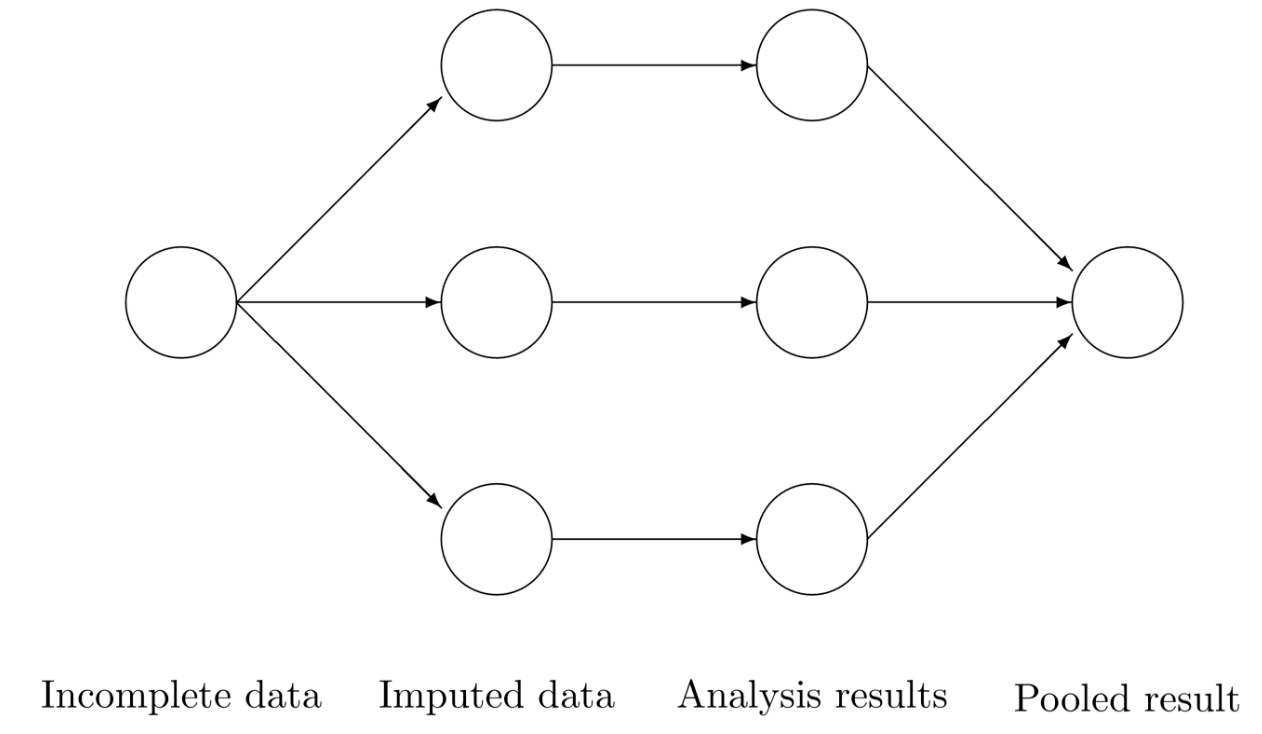
\includegraphics[width=400px]{figure/multiple-imputation-workflow} 

}

\caption{Multiple Imputation Workflow}\label{fig:mutlipleimputationworkflow}
\end{figure}
Based on the data, use-case, and desired outcome, practitioners should
choose an imputation method that adds some random variation. Then
multiple imputation results in multiple copies of imputed datasets with
different imputed values. Each imputed dataset is analyzed separately
and then parameters from those analyses are pooled together to get
combined diagnostics on the performance of the multiple imputation
process and the specified imputation model. This method ``solves the
standard error problem by calculating the variance of each parameter
estimate across the several data sets'' (Allison, 2012). The pooled
parameters replace those from the supervised machine learning model of
interest. The pooled parameters not only produce the coefficient
estimate but also the properly account for the increase in standard
error due to uncertainty introduced from imputing missing data.

\section*{Missing Data and
Autoimpute}\label{background-missing-data-autoimpute}
\addcontentsline{toc}{section}{Missing Data and Autoimpute}

Ultimately, this background details the concepts and theory that are the
foundation for the Autoimpute package. Understanding the process that
generates missingness in a dataset - the missing data mechanism - is
imperative prior to applying any deletion or imputation method. The
missing data mechanism and missing data pattern should inform which
strategy to use to handle missing data. At that point, the researcher
performs either univariate or multivariate imputation using the method
that fits best a given dataset, use case, or goal. If the researcher is
interested in analysis, then he or she should deploy the selected
imputation method in multiple imputations. Each imputed dataset within
the multiple imputation framework can then be analyzed separately with
the supervised learning model of interest. Finally, the researcher can
pool parameters together to produce parameters of the multiply imputed
analysis model and use this model to make predictions when new data
arrives.

Anyone interested can utilize \texttt{Autoimpute}, the Python package
created by the authors, to perform all of the steps described above. The
next section discusses how to use \texttt{Autoimpute} from end-to-end to
explore and analyze missing data. It also demonstrates the impact
different missing data mechanisms have on the results produced from
multiple imputation and subsequent analysis. All results are generated
using the \texttt{Autoimpute} package.

\chapter*{Methodology}\label{methodology}
\addcontentsline{toc}{chapter}{Methodology}

In this section, the researchers use \texttt{Autoimpute} to demonstrate
its capabilities as an end-to-end framework for analyzing datasets with
missing values. The researchers showcase the package's features on two
datasets with different types of missingness.

The researchers begin by simulating a dataset with no missingness. A
simple linear regression is performed on this simulated dataset and its
coefficients are stored as benchmarks for comparison of all future
analysis models. Then, in each example, the researchers introduce
missingness within the given dataset using a predefined missingness
mechanism. This dataset with missing values becomes the source of truth
for deletion and imputation methods performed on the simulated missing
data.

In each example, the researchers then explore missingness patterns
within the dataset. After exploration, they employ complete-case
analysis or listwise deletion. Following this procedure, they use the
missing value dataset to create imputations based on a number of
imputation methods. They use univariate imputation methods including
mean imputation and multivariate methods including least squares and
predictive mean matching. They then run the processed missing value
datasets through a simple linear regression and gather the respective
coefficients and feature variance for comparison. Lastly, they compare
the results to see the impact of deletion and imputation on the
analytical model under the circumstances described in each example.

\section*{The Full Dataset}\label{the-full-dataset}
\addcontentsline{toc}{section}{The Full Dataset}

The full dataset contains 500 observations for feature \(x\) and
response \(y\). Both datasets come from a joint multivariate normal
distribution, and the correlation between \(x\) and \(y\) is \(0.5\).
The mean of each distribution is zero.

The figure below describes each feature within the distribution:
\begin{figure}

{\centering 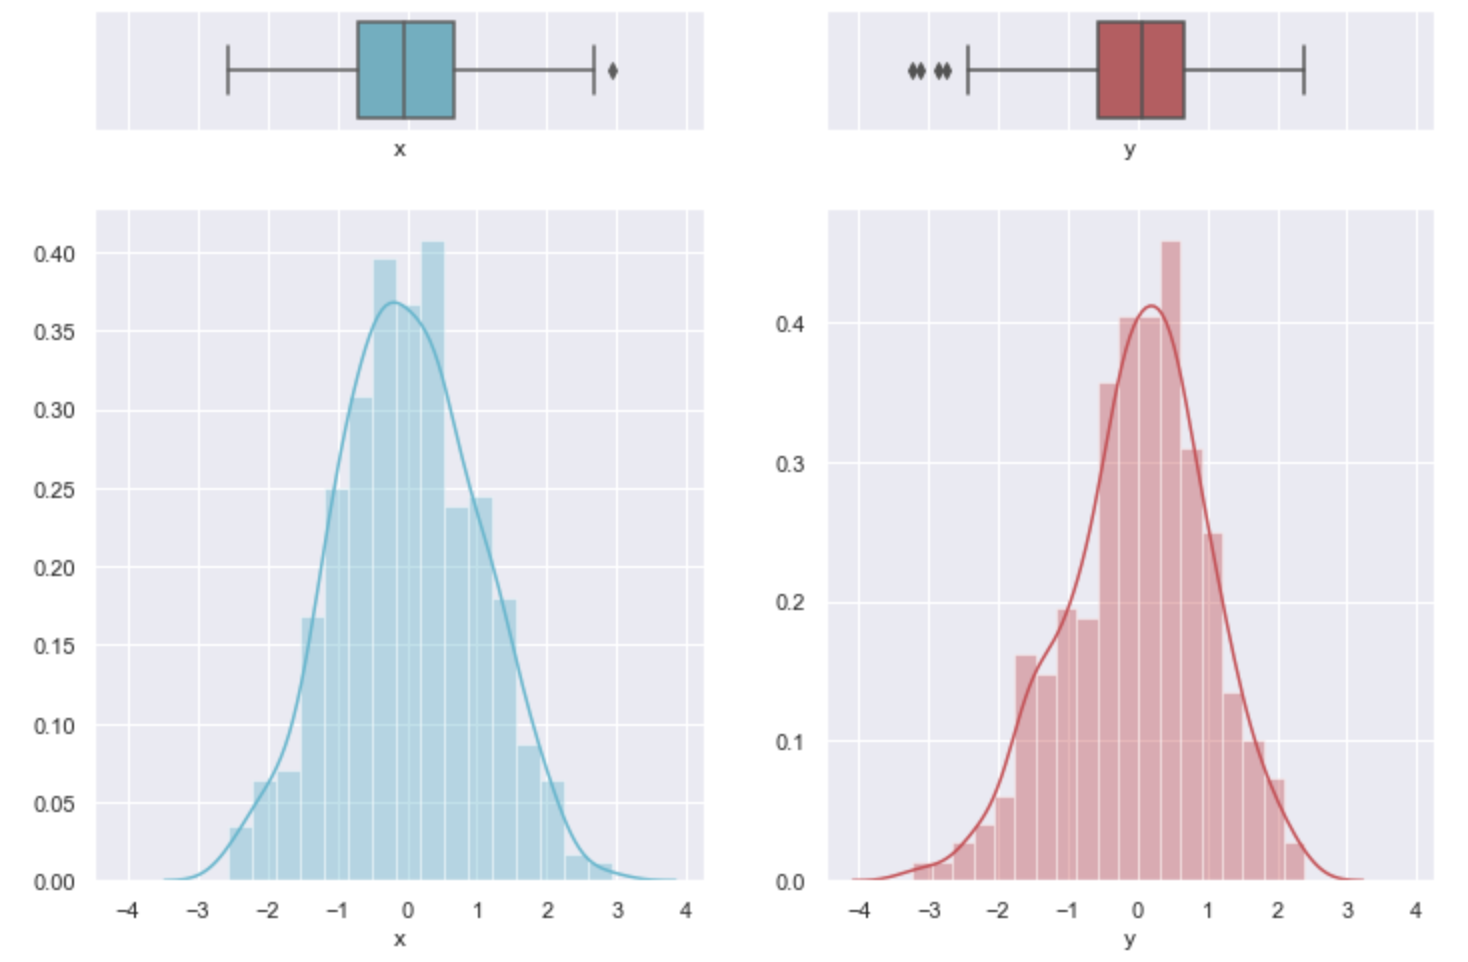
\includegraphics[width=300px]{figure/full-side-by-side} 

}

\caption{Distribution of Full x and y}\label{fig:fullsidebyside}
\end{figure}
The next figure demonstrates the joint relationship between each
feature, with the marginals plotted as well:
\begin{figure}

{\centering 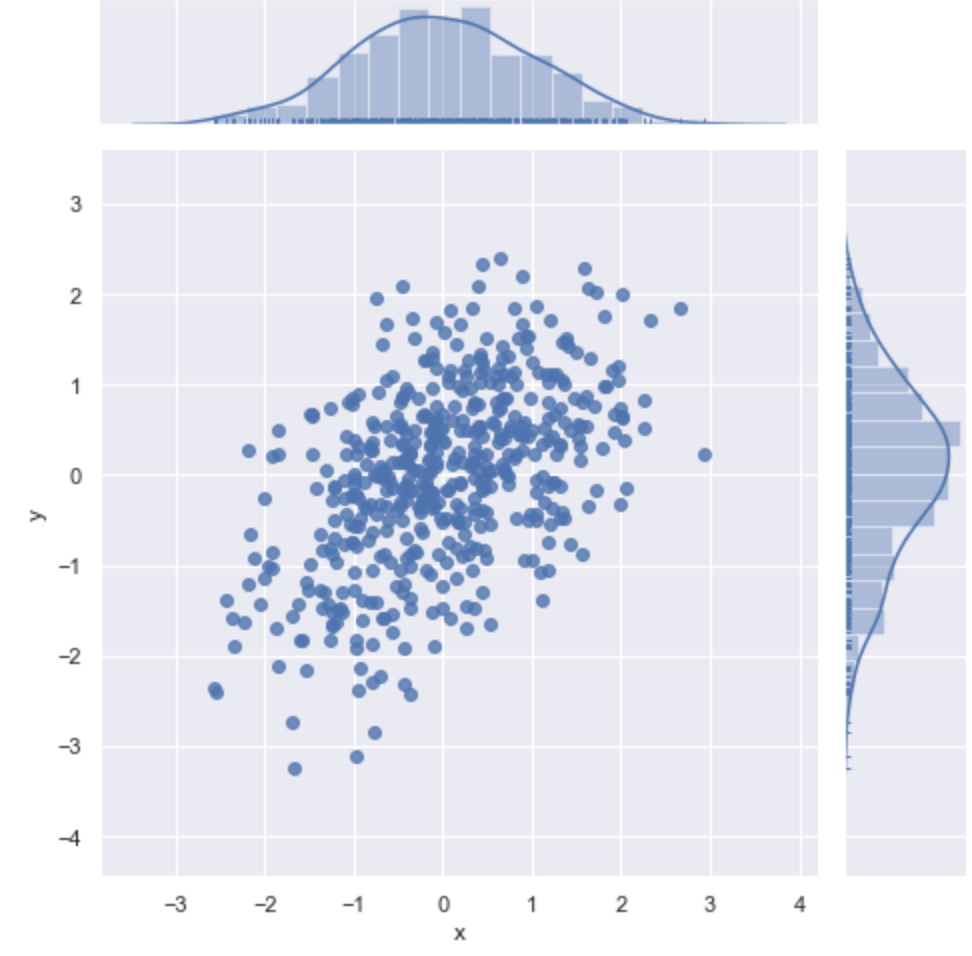
\includegraphics[width=300px]{figure/full-joint} 

}

\caption{Joint and Marginals of Full x and y}\label{fig:full-joint}
\end{figure}
The full dataset does not contain any missing values. Therefore, we do
not have to perform any imputation before we conduct analysis. Using
\texttt{Autoimpute}, the researchers perform linear regression on the
full dataset. The results appear below:
\begin{figure}

{\centering 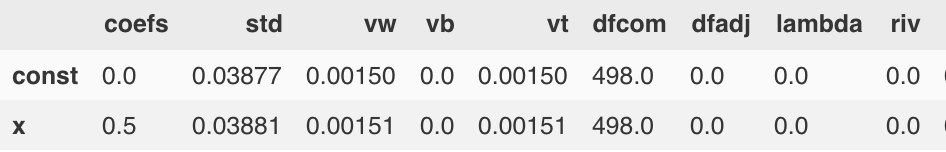
\includegraphics[width=300px]{figure/full-regression} 

}

\caption{Linear Regression Results: Full}\label{fig:full-regression}
\end{figure}
The results from linear regression on the full dataset serve as the
golden source.

The output above displays for each variable the following:
\begin{itemize}
\tightlist
\item
  \texttt{coefs} - Linear regression coefficients for each variable\\
\item
  \texttt{std} - The standard error of the coefficient estimate\\
\item
  \texttt{vw} - The variance of the coefficient within each
  complete-data sample\\
\item
  \texttt{vb} - The variance between each complete-data sample\\
\item
  \texttt{vt} - The total variance including vw, vb \& extra simulation
  variance\\
\item
  \texttt{dfcom} - The degrees of freedom for the hypothetically
  complete dataset\\
\item
  \texttt{dfadj} - Adapted degrees of freedom for smaller sample sizes\\
\item
  \texttt{lambda} - The proportion of variance due to nonresponse\\
\item
  \texttt{riv} - The relative increase in variance
\end{itemize}
Observe that \texttt{vb}, \texttt{lambda}, and \texttt{riv} are all
equal to 0. This result occurs because no imputation is necessary and no
multiple imputation takes place. Therefore, we focus mainly on the
\texttt{coefs} and \texttt{std} results from above as benchmarks for
comparison in the analysis from each example below. These additional
metrics become important when we observe examples that contain multiple
imputations.

\section*{Example 1: MCAR with Missingness in the
Response}\label{example-1-mcar-with-missingness-in-the-response}
\addcontentsline{toc}{section}{Example 1: MCAR with Missingness in the
Response}

In the first example, the researchers generate MCAR missingness within
the response, \(y\). Response \(y\) contains 40\% missing values.
Feature \(x\) remains fully observed. The two plots below showcase how
to use \texttt{Autoimpute} to explore missingness within a given
dataset. The plots are quite simple in this case, but they can help
detect patterns in missing data when multiple features are present with
different levels of missingness.
\begin{figure}

{\centering 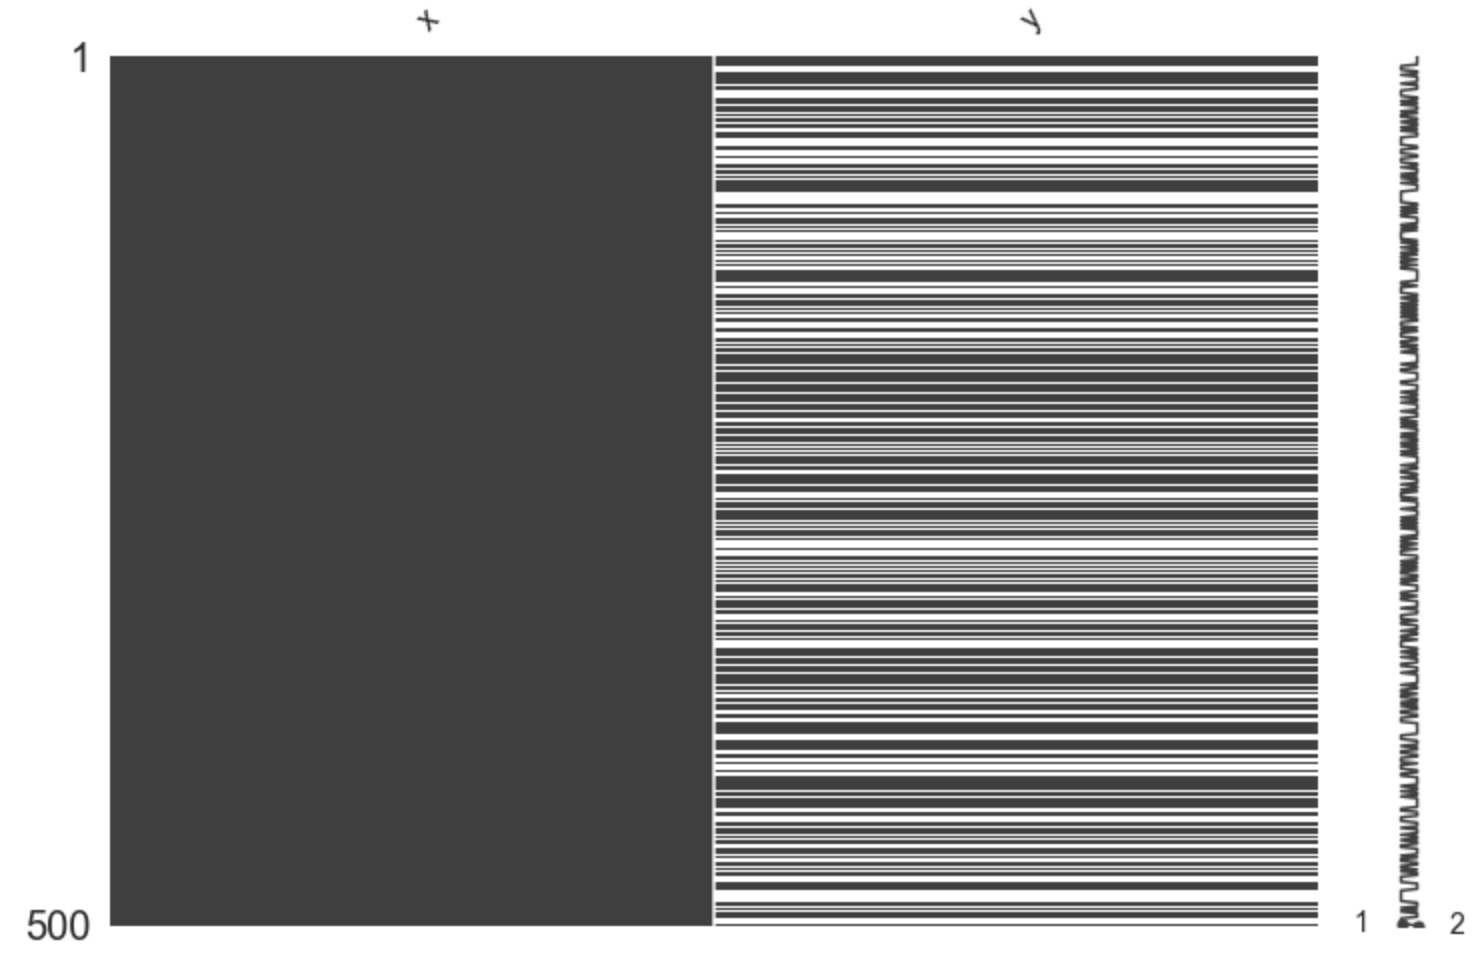
\includegraphics[width=300px]{figure/y-mis-forty-loc} 

}

\caption{Missingness Locations}\label{fig:y-mis-forty-loc}
\end{figure}
\begin{figure}

{\centering 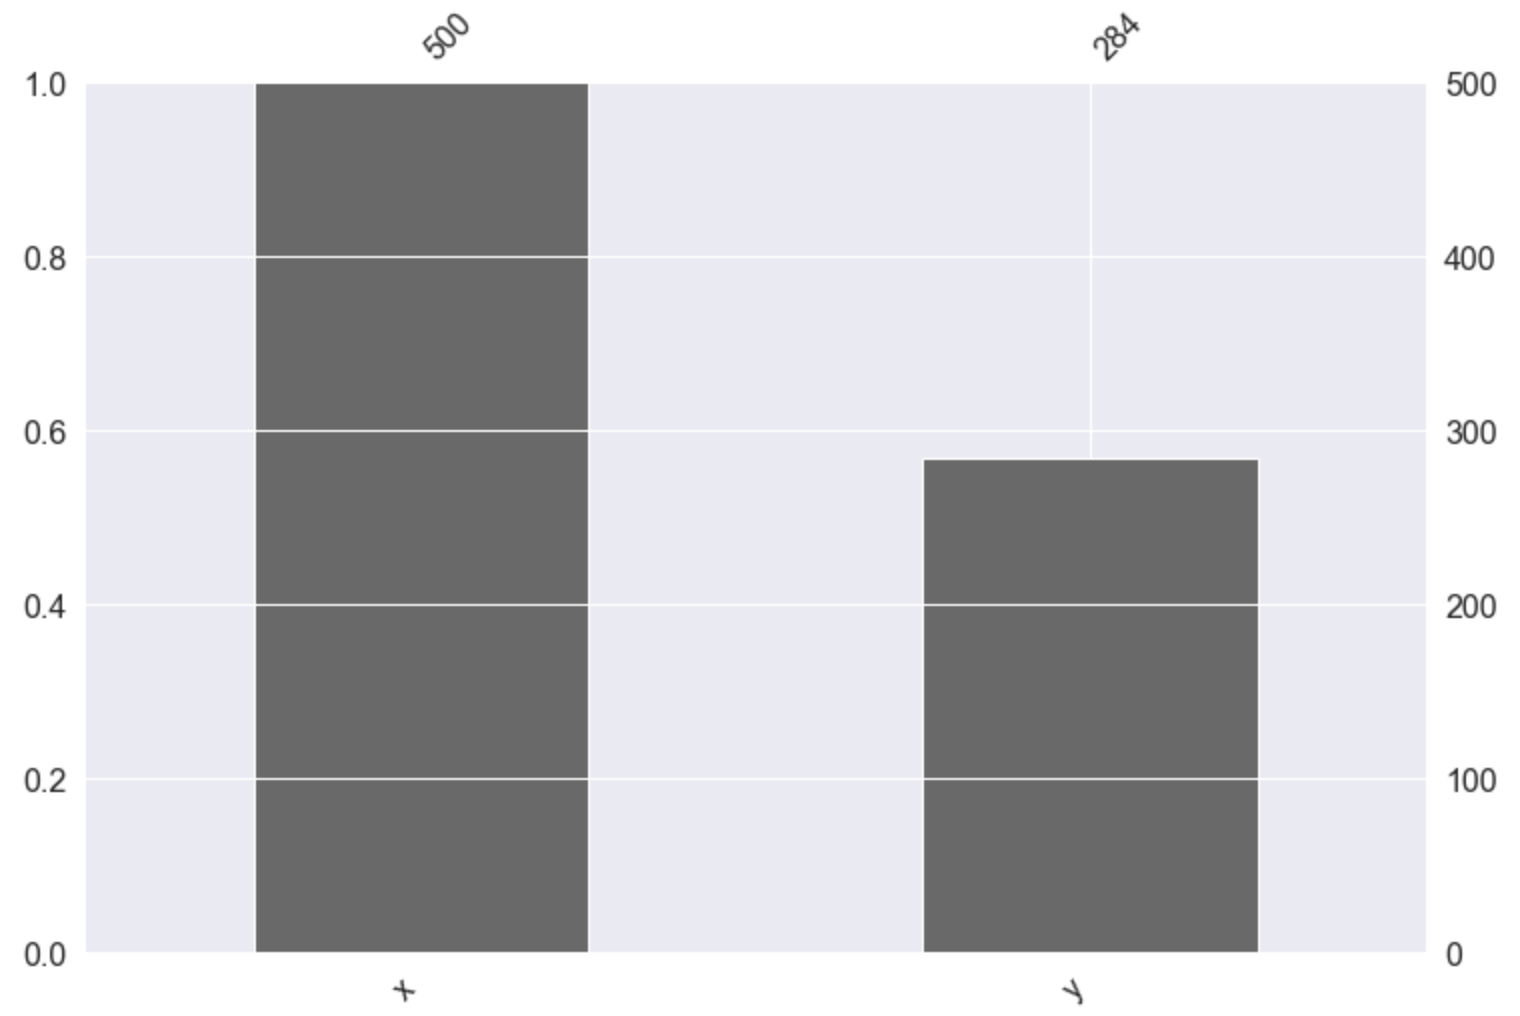
\includegraphics[width=300px]{figure/y-mis-forty-bar} 

}

\caption{Missingness Percentage}\label{fig:y-mis-forty-bar}
\end{figure}
Next, the researchers employ missing data methods to handle missing
data. In this case, missing data methods must find plausible imputations
for the 40\% of \(y\) that is missing. The imputation methods used
include mean, linear regression, and pmm. The researchers also use
listwise deletion, although there is no visualization within
\texttt{Autoimpute} for complete-case analysis because no imputations
are performed. For imputation methods, the researchers deploy each
strategy within the multiple imputation framework. The number of
imputations performed for each method is 5.

The visualizations below show the impact of mean, linear regression, and
pmm. For each strategy, there are two respective plots. The first plot
is the new multivariate distribution between \(x\) and \(y\) after
imputation. The second plot is a swarm plot that shows the imputations
for \(y\) against other, observed values for \(y\) for each of the \(5\)
imputations performed.

Let's start with mean imputation:
\begin{figure}

{\centering 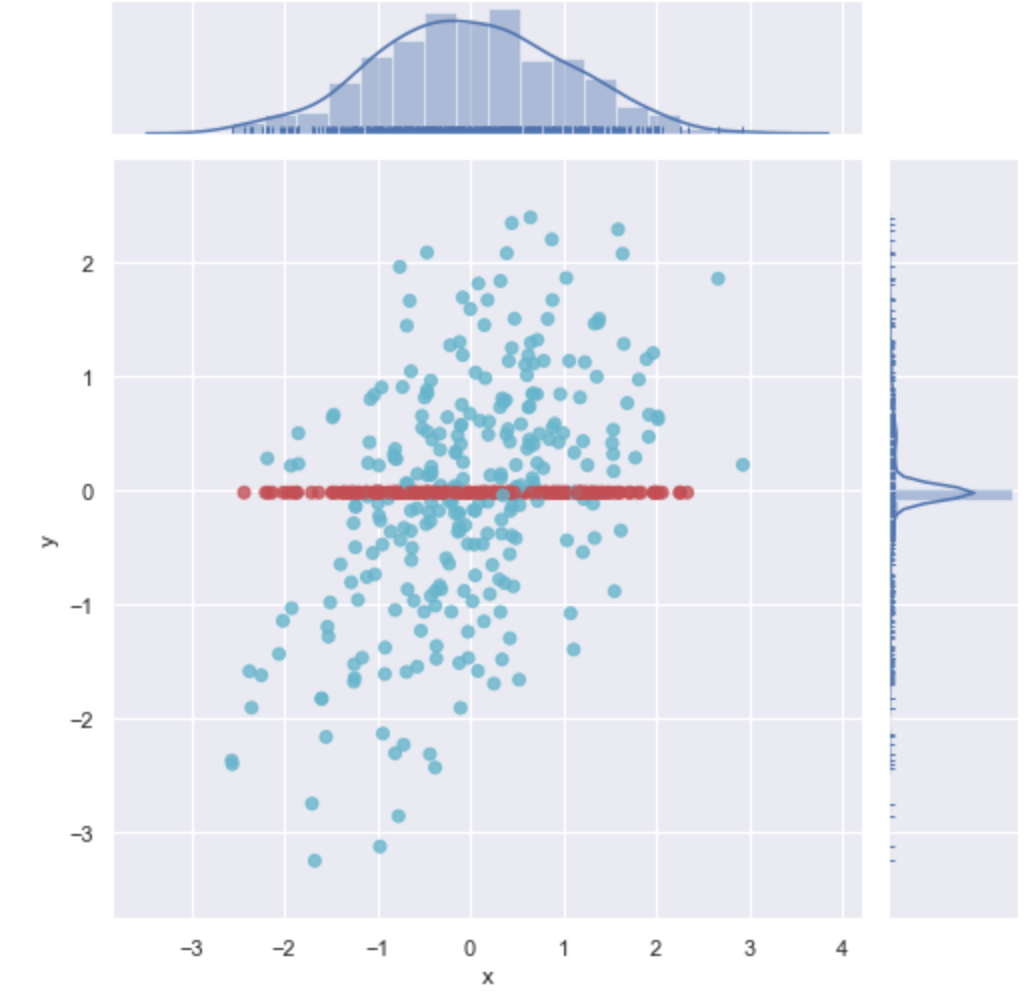
\includegraphics[width=300px]{figure/multi-mean} 

}

\caption{Joint and Marginals with Mean Imputation}\label{fig:multi-mean}
\end{figure}
\begin{figure}

{\centering 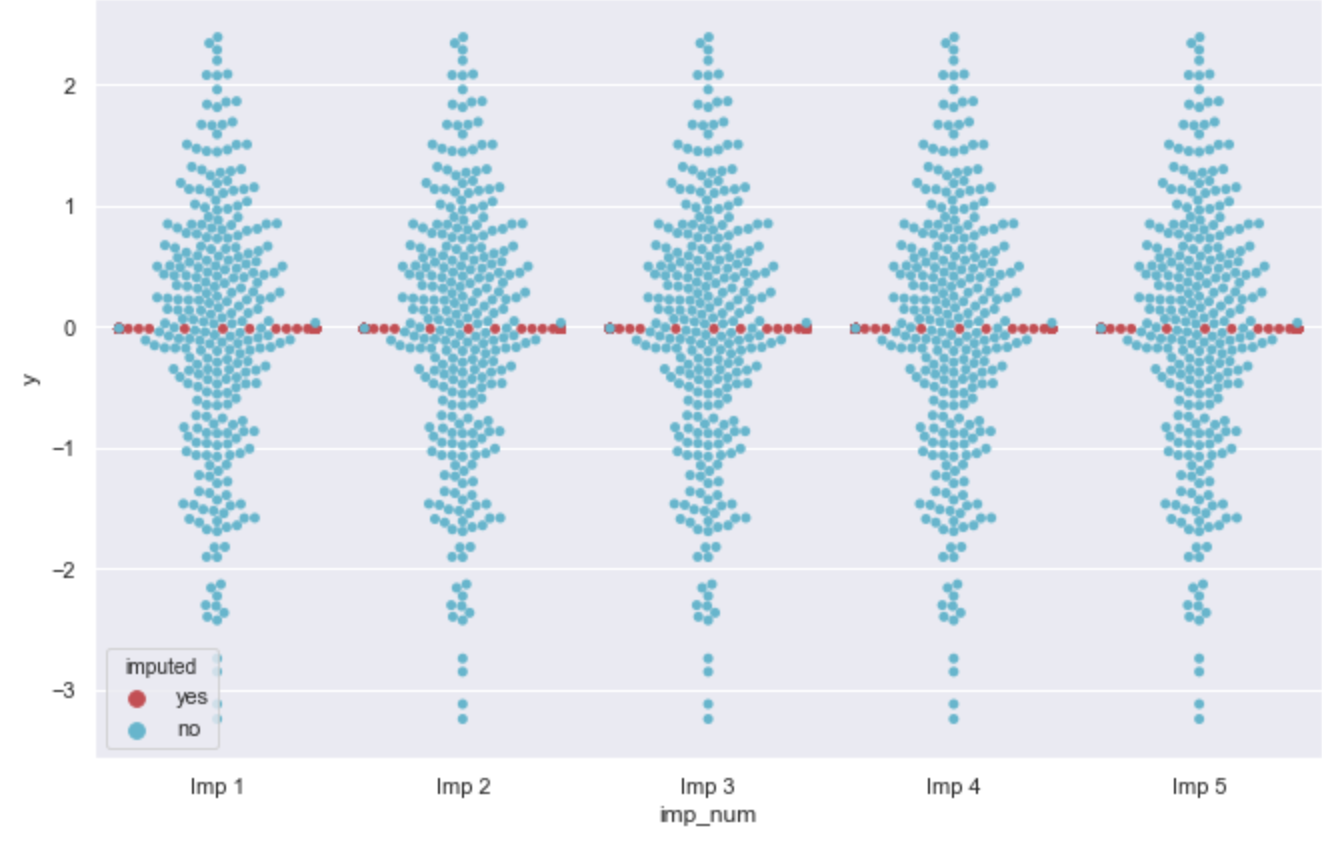
\includegraphics[width=300px]{figure/swarm-mean} 

}

\caption{Swarm Plot: Mean Imputation}\label{fig:swarm-mean}
\end{figure}
Note that for mean imputation, the imputations do not depend on the
value of \(x\), and the relationship between \(y\) and \(x\) is ignored.
This result makes sense, as mean imputation is a univariate method. Also
note that the imputation values in the swarm plot are the same for each
imputation. This occurs because the mean of the observed values of \(y\)
do not change from imputation to imputation within the multiple
imputation framework. Therefore, the imputation values within each
imputed dataset are the same, and the imputation values accross each
imputed dataset are the same.

Next, observe imputation via least squares:
\begin{figure}

{\centering 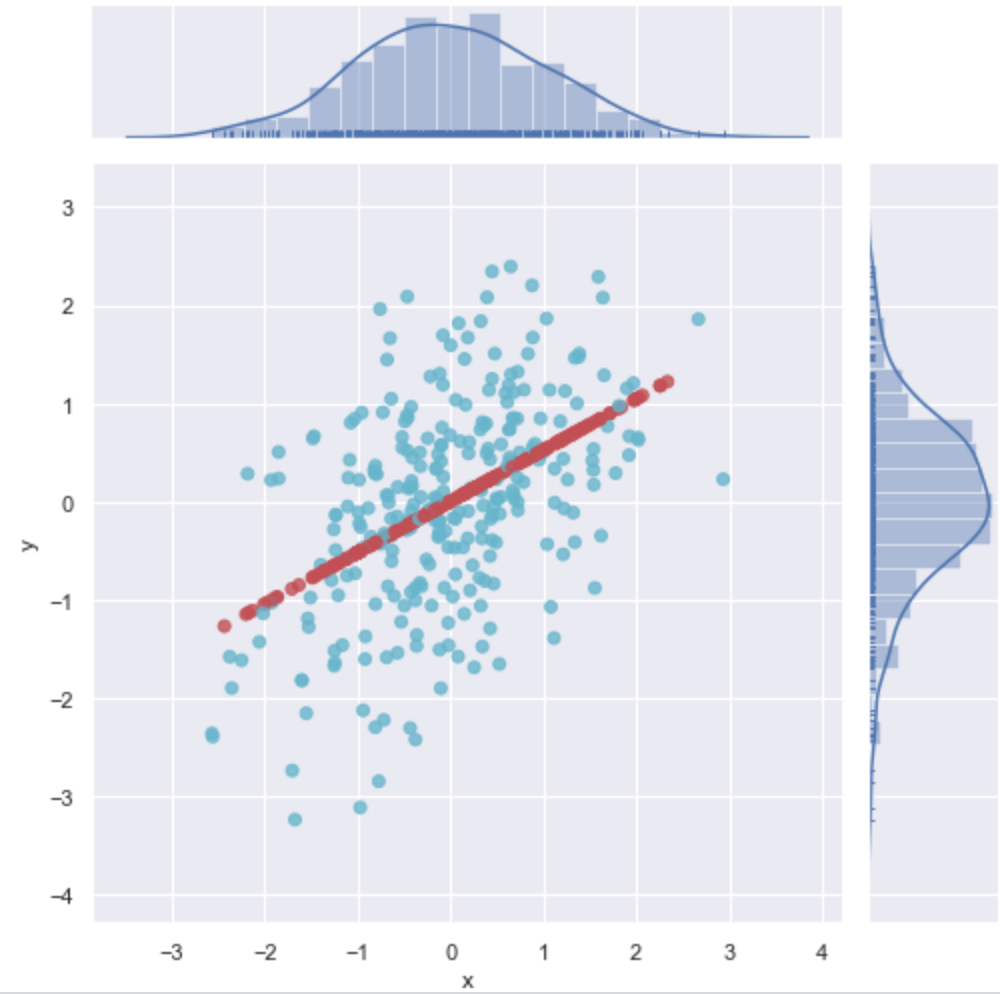
\includegraphics[width=300px]{figure/multi-lm} 

}

\caption{Joint and Marginals with Least Squares Imputation}\label{fig:multi-lm}
\end{figure}
\begin{figure}

{\centering 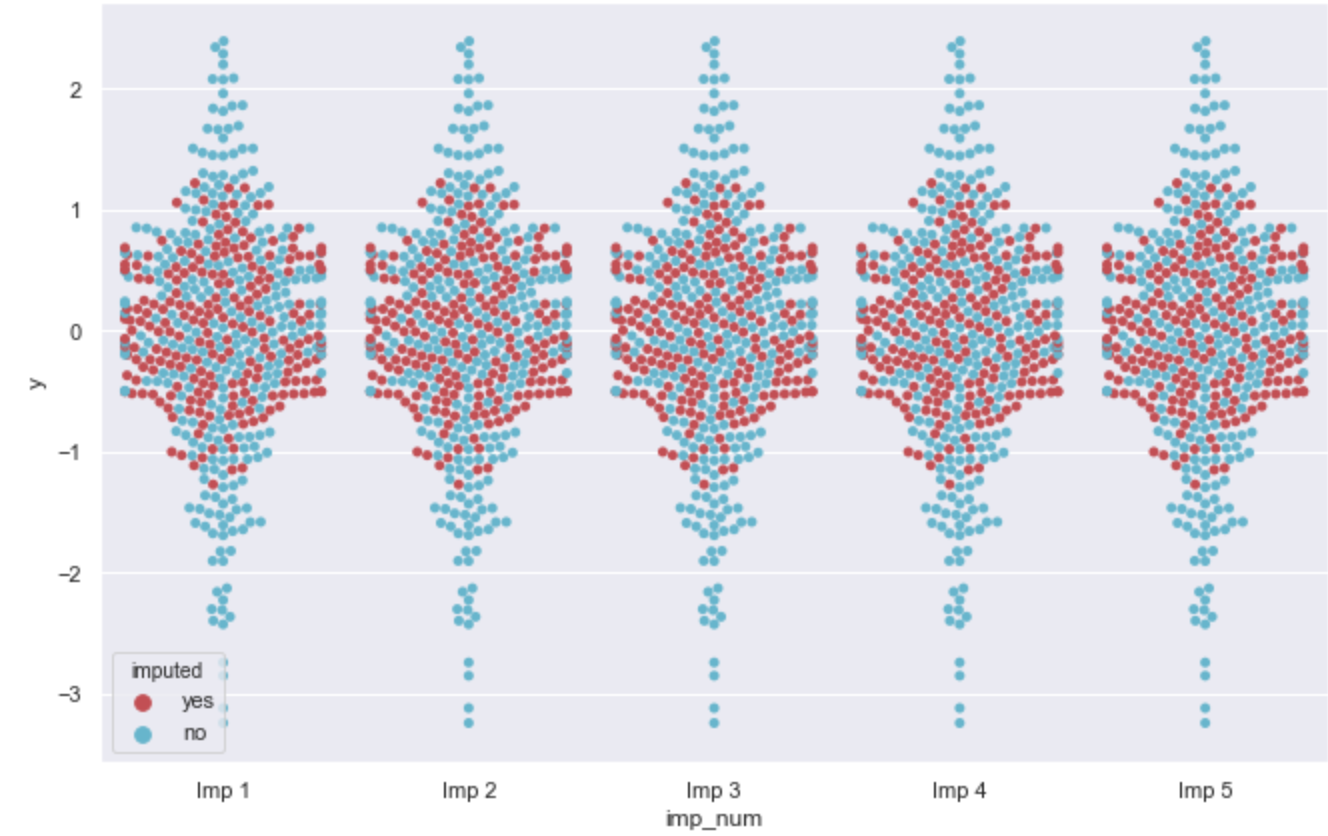
\includegraphics[width=300px]{figure/swarm-lm} 

}

\caption{Swarm Plot: Least Squares Imputation}\label{fig:swarm-lm}
\end{figure}
The plots for linear regression now take into account the relationship
between \(y\) and \(x\). As a result, the imputed values are different
within imputations but the same across imputations. Within imputations,
the linear model produces different results, which depend on the value
of \(x\). But across imputations, the linear model is the same because
it is fit to the same data and no random error is added to imputations.

Finally, observe pmm imputation:
\begin{figure}

{\centering 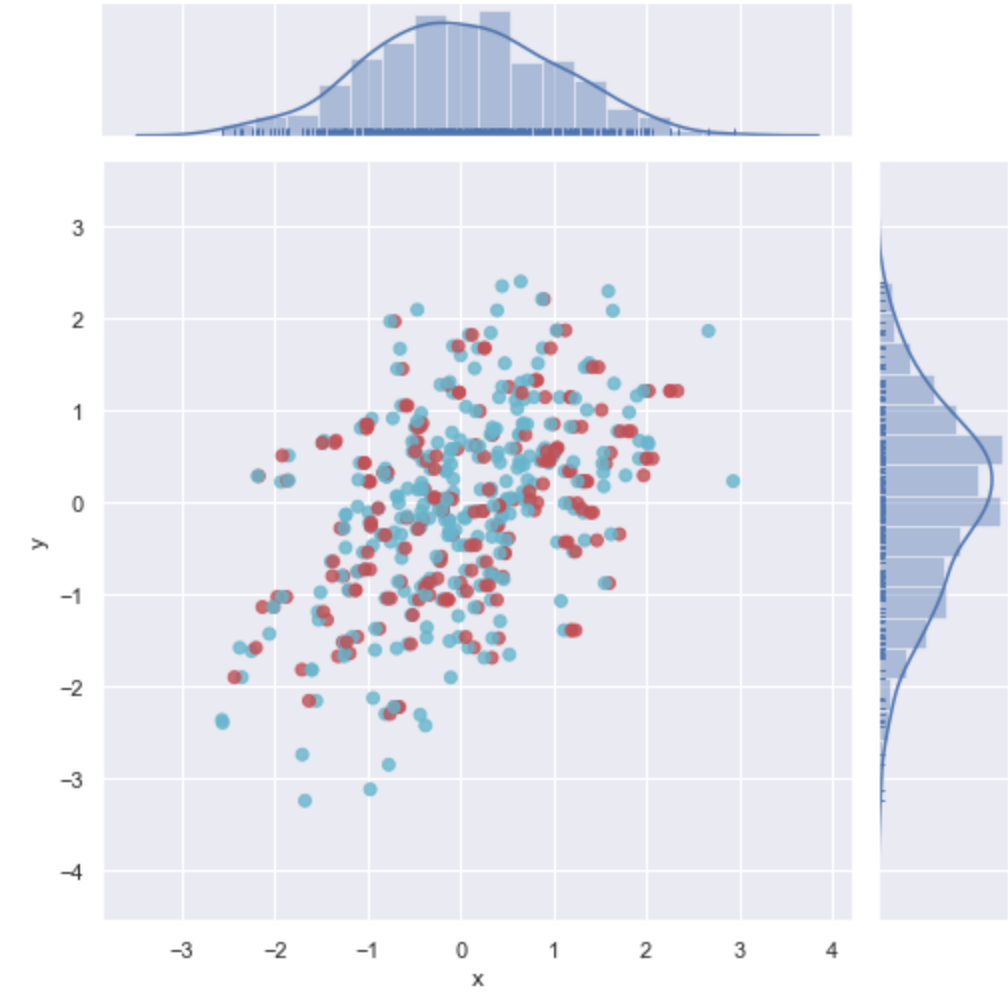
\includegraphics[width=300px]{figure/multi-pmm} 

}

\caption{Joint and Marginals with PMM Imputation}\label{fig:multi-pmm}
\end{figure}
\begin{figure}

{\centering 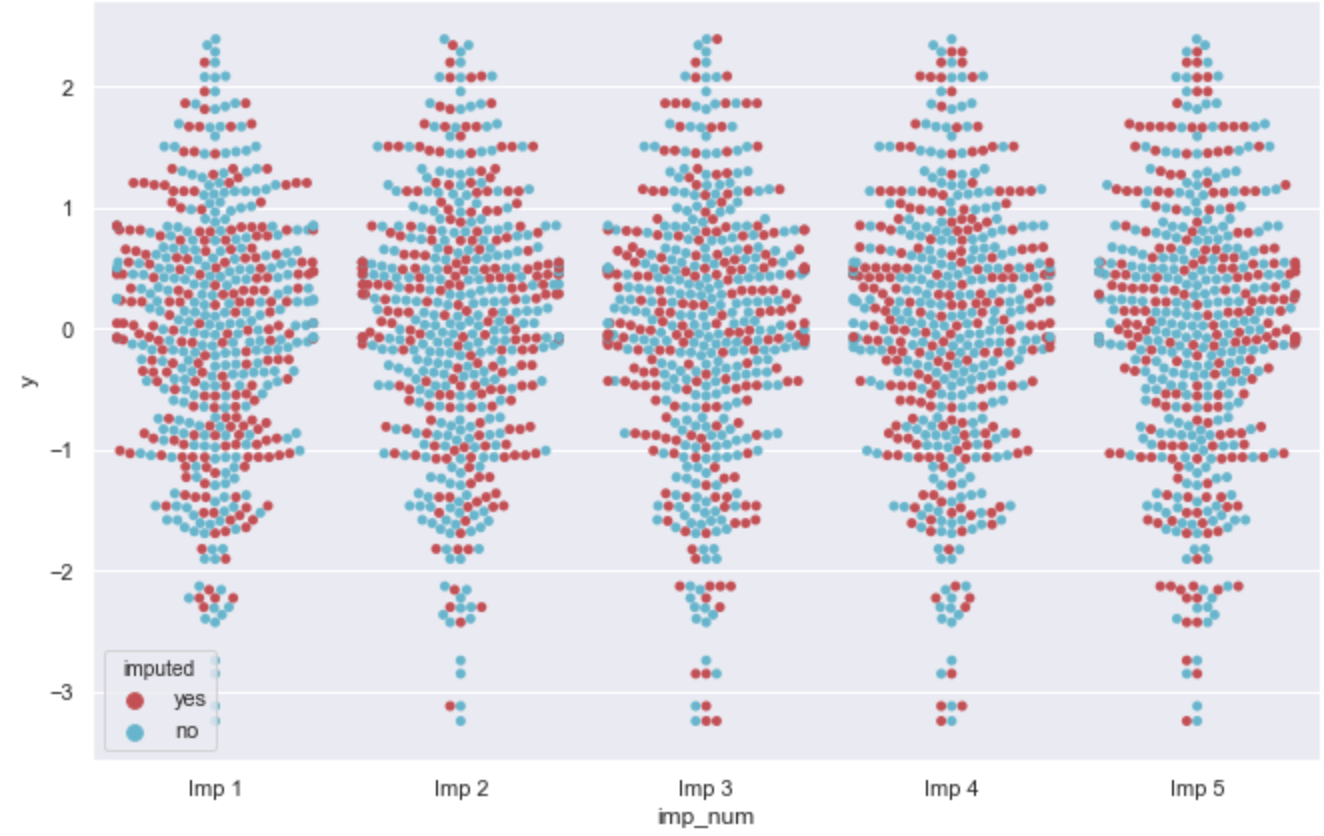
\includegraphics[width=300px]{figure/swarm-pmm} 

}

\caption{Swarm Plot: PMM Imputation}\label{fig:swarm-pmm}
\end{figure}
PMM Imputation respects not only the relationship between \(y\) and
\(x\) but also the variance between the features. Imputations are no
longer from the ``line of best fit'' as they are with linear regression.
Additionally, imputations are different within and across imputations.
Therefore, PMM does the best job at respecting the structure of the data
and adding variance between / across imputed datasets.

\section*{Example 2: MAR with Missingness in the
Predictor}\label{example-2-mar-with-missingness-in-the-predictor}
\addcontentsline{toc}{section}{Example 2: MAR with Missingness in the
Predictor}

In the second example, the researchers generate MAR missingness within
the predictor, \(x\). Predictor \(x\) contains 40\% missing values.
Response \(y\) remains fully observed. To keep this section concise, we
will not generate the same plots that we did above, but we will apply
the exact same methods. \texttt{Autoimpute} can impute both features and
predictors, and it can examine missingness anywhere it exists within a
dataset.

The researchers take the same approach to Example 2 as they do to
Example 1. Multiple imputation is performed, with the number of
imputations equal to 5. The same methods are applied as well (listwise
delete, mean, least squares, and pmm).

\section*{Analysis Models on each
Example}\label{analysis-models-on-each-example}
\addcontentsline{toc}{section}{Analysis Models on each Example}

The sections above take the user through the data exploration phase and
multiple imputation phase of \texttt{Autoimpute}. The next section,
Findings, demonstrates how the nature of missingness affected the
results of linear regression on our mulitply imputed data.

\chapter*{Findings}\label{findings}
\addcontentsline{toc}{chapter}{Findings}

\section*{Full Model Recap}\label{full-model-recap}
\addcontentsline{toc}{section}{Full Model Recap}

We begin this section with a recap of linear regression on the full
dataset. The results below serve as the benchmark for comparison. They
are considered the golden standard. Therefore, we seek to examine how
our imputation methods perform and if they produce a dataset that
significantly affects the results from linear regression. If the results
are skewed, we know that the imputation model used is significantly
affected by the nature of missingness within the data, and we may have
to do more to account for the missingness.

The results for the full model are displayed below:
\begin{figure}

{\centering 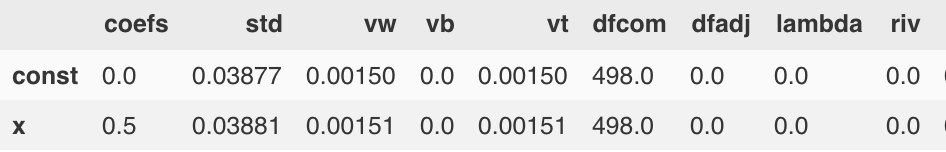
\includegraphics[width=300px]{figure/full-regression} 

}

\caption{Linear Regression Results: Full}\label{fig:full-regression-again}
\end{figure}
\section*{Results from Example 1}\label{results-from-example-1}
\addcontentsline{toc}{section}{Results from Example 1}

Next, we examine the results from a linear regression on the imputed
dataset from Example 1. Recall that Example 1 contains 40\% missingness
in the response \(y\), and the missingness mechanism is MCAR.

First, listwise delete:
\begin{figure}

{\centering 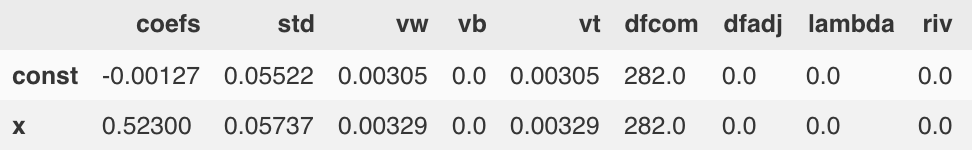
\includegraphics[width=300px]{figure/mcar-listwise-delete} 

}

\caption{Linear Regression Results: Listwise Delete}\label{fig:mcar-listwise-delete}
\end{figure}
Next, mean imputation:
\begin{figure}

{\centering 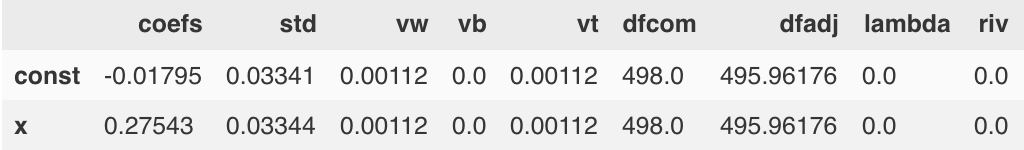
\includegraphics[width=300px]{figure/mcar-mean} 

}

\caption{Linear Regression Results: Mean Imputation}\label{fig:mcar-mean}
\end{figure}
Next, least squares imputation:
\begin{figure}

{\centering 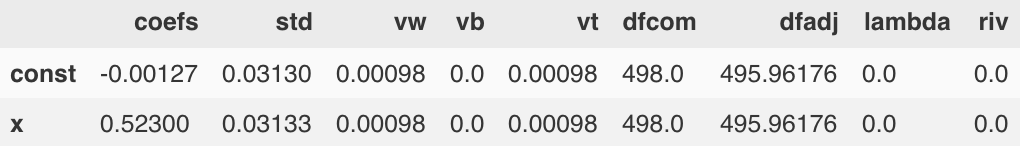
\includegraphics[width=300px]{figure/mcar-ls} 

}

\caption{Linear Regression Results: Least Squares Imputation}\label{fig:mcar-ls}
\end{figure}
Finally, pmm imputation:
\begin{figure}

{\centering 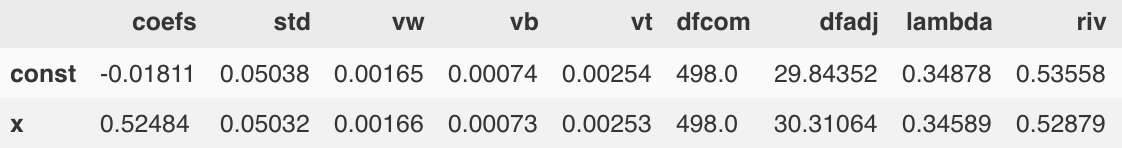
\includegraphics[width=300px]{figure/mcar-pmm} 

}

\caption{Linear Regression Results: PMM Imputation}\label{fig:mcar-pmm}
\end{figure}
\section*{Results from Example 2}\label{results-from-example-2}
\addcontentsline{toc}{section}{Results from Example 2}

Next, we examine the results from a linear regression on the imputed
dataset from Example 2. Recall that Example 2 contains 40\% missingness
in the predictor \(x\), and the missingness mechanism is MAR.

First, listwise delete:
\begin{figure}

{\centering 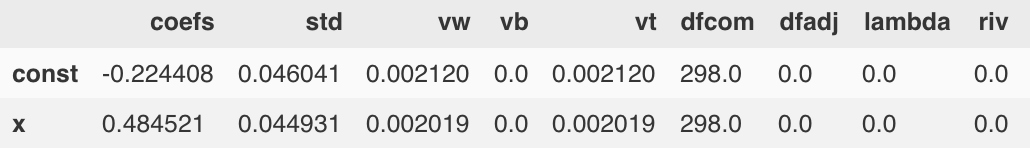
\includegraphics[width=300px]{figure/mar-listwise-delete} 

}

\caption{Linear Regression Results: Listwise Delete}\label{fig:mar-listwise-delete}
\end{figure}
Next, mean imputation:
\begin{figure}

{\centering 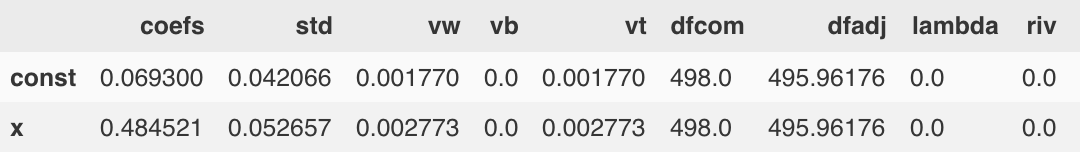
\includegraphics[width=300px]{figure/mar-mean} 

}

\caption{Linear Regression Results: Mean Imputation}\label{fig:mar-mean}
\end{figure}
Next, least squares imputation:
\begin{figure}

{\centering 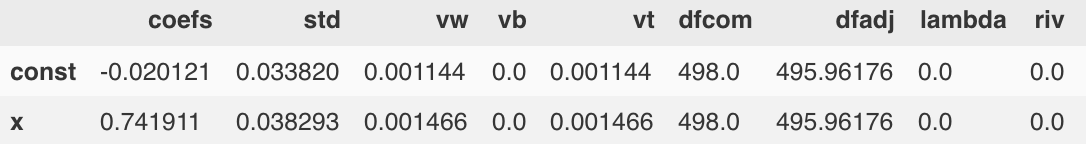
\includegraphics[width=300px]{figure/mar-ls} 

}

\caption{Linear Regression Results: Least Squares Imputation}\label{fig:mar-ls}
\end{figure}
Finally, pmm imputation:
\begin{figure}

{\centering 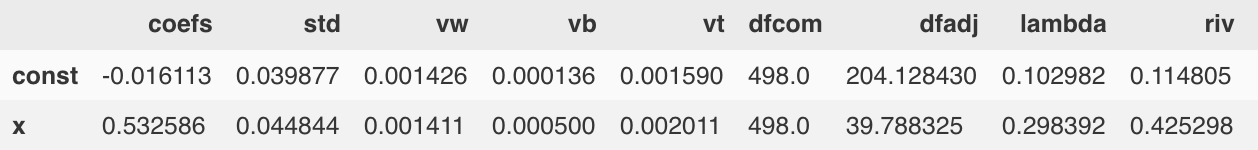
\includegraphics[width=300px]{figure/mar-pmm} 

}

\caption{Linear Regression Results: PMM Imputation}\label{fig:mar-pmm}
\end{figure}
\section*{Analysis of Results}\label{analysis-of-results}
\addcontentsline{toc}{section}{Analysis of Results}

We see that regardless of the missing data mechanism, mean and least
squares imputation significantly reduce the variance in the coefficient
estimates. Therefore, these methods should be avoided regardless because
they significantly overstate the confidence we have in an estimate's
coefficient. When missingness is in the predictor, least squares is
quite biased. When missingness is in the response, mean is biased
downward as well. When data is MCAR, listwise deletion is the most
efficient and therefore preferred. When data is MAR, listwise deletion
becomes slightly biased, and PMM is the most robust.

\chapter*{Conclusion}\label{conclusion}
\addcontentsline{toc}{chapter}{Conclusion}

In summary, this project examines the nature of missingness and provides
an end-to-end methodology for missing data \& imputation analysis. It
focuses on four key objectives: describe and visualize the extent of the
missing value problem; examine factors related to missingness; develop
methods to impute missing data; and measure the impact of imputation on
inference derived from supervised learning, specifically linear
regression. The researchers create a open-source, Python-based package
called Autoimpute to accomplish these objectives. The Autoimpute package
provides methods to explore missingness, implement imputation methods,
and analyze their impact on analytical models in a flexible way. This
report specifically focuses on establishing a solid foundation around
the concepts missing data \& imputation and demonstrates examples of
missing data analysis with different types of missing data. Ultimately,
this research provides python-focused data practitioners a tool to use
to explore missingness in their datasets, perform imputation methods,
and assess the impact of imputation on analytical models downstream.

\chapter*{Recommendations}\label{recommendations}
\addcontentsline{toc}{chapter}{Recommendations}

This research explores missingness and outlines a framework through
which a data practitioner can conduct missing data and imputation
analysis. The researchers recommend data practitioners use the
flexibility, simplicity, and granularity of the Autoimpute package to
conduct their own missing data analyses. To start, data practitioners
should review the Autoimpute package tutorials (See Appendix A.0) and
get a better understanding of how the package works. This will help data
practitioners follow best practices when utilizing the package. Once
that is clear, data practitioners should clone the publicly available
package from GitHub (See Appendix A.0) and start their analyses. If
issues arise during your analyses, please contact the researchers.
Lastly, the researchers ask that you share your feedback about the
Autoimpute package or any interesting results you find in your analyses.

\appendix

\chapter{Autoimpute References}\label{autoimpute-references}

\chapter{Notation Cheatsheet}\label{notation-cheatsheet}

\chapter{Concepts Related to
Missingness}\label{concepts-related-to-missingness}

\chapter{Univariate Imputation
Methods}\label{univariate-imputation-methods}

\chapter{Multivariate Imputation
Methods}\label{multivariate-imputation-methods}

\backmatter

\chapter*{References}\label{references}
\addcontentsline{toc}{chapter}{References}

Allison, P. D. (2012). Handling Missing Data by Maximum Likelihood. SAS
Global Forum 2012. Retrieved April 23, 2019, from\\
\url{https://statisticalhorizons.com/wp-content/uploads/MissingDataByML.pdf}.

Economic Commission for Europe of the United Nations (UNECE) (2000),
``Glossary of Terms on Statistical Data Editing'', Conference of
European Statisticians Methodological material, Geneva.

Gelman, A., \& Hill, J. (2017). Data analysis using regression and
multilevel/hierarchical models. Cambridge: Cambridge University Press.

Introduction to SAS (2017). UCLA: Statistical Consulting Group. From
\url{https://stats.idre.ucla.edu/sas/modules/sas-learning-moduleintroduction-to-the-features-of-sas/}
(accessed April, 21, 2019).

Morris, T. P., White, I. R., \& Royston, P. (2014). Tuning multiple
imputation by predictive mean matching and local residual draws. BMC
Medical Research Methodology, 14(1).
\url{https://doi.org/10.1186/1471-2288-14-75}

Nakagawa, S. (2015). CHAPTER 4 Missing data : mechanisms , methods , and
messages.

Rubin, D. B. (1976)., Inference and missing data, Biometrika, Volume 63,
Issue 3, Pages 581--592, \url{https://doi.org/10.1093/biomet/63.3.581}

Van Buuren, S. (2018). Flexible imputation of missing data. Boca Raton:
Chapman \& Hall/CRC.

Yu, A., Wagner, J. T., \& Murugesan, M. (2017). Comparative Evaluation
of Recent ML Based Missing Data Imputation Methods with NORC's Survey of
Consumer Finances. University of Chicago Graham School. Retrieved
November 1, 2018.


% Index?

\end{document}
